%% ----------------------------------
%%   Kap05---Evaluation.tex
%% ----------------------------------

%% zeigen, dass der in Kap. 4 gebaute Prototyp auch wirklich funktioniert (Laufzeitmessungen, Fotos, Screenshots, ...)
%% Welche Punkte der Zielsetzung wurden nicht erreicht?

\chapter{Evaluation}
\label{sec:Chapter5}
Dieses Kapitel evaluiert die Ergebnissen dieser Arbeit. Der Output der automatischen Qualitätsbestimmung von Memristoren wurde bereits im vorherigen Kapitel~\ref{sec:Chapter4} dargestellt. Die Messungen, welche eine wiederholte Qualitätsbestimmung eines Memristors und den dazugehörigen Output darstellen, werden in den folgenden Abschnitten diskutiert und erklärt.

\section{Die Ergebnisse}
Der Output der Implementierung wurde für Evaluationszwecke in der folgenden Form dargestellt (siehe Tabellen~\ref{tab:Messergebnisse_Sn},~\ref{tab:Messergebnisse_W},~\ref{tab:Messergebnisse_Cr}~und~\ref{tab:Messergebnisse_old}):
\begin{description}
  \item[f-Grade: ] Die Note für die Formbarkeit des getesteten Memristors.
  \item[t-Grade: ] Die Note für den Energieverbrauch, abhängig von dem Threshold des getesteten Memristors.
  \item[s-Grade: ] Die Note für die Speichergröße des getesteten Memristors.
  \item[Grade: ] Die Gesamtnote des getesteten Memristors.
  \item[minLT: ] die minimale Restlebensdauer des getesteten Memristors.
  \item[typLT:] die typische Restlebensdauer des getesteten Memristors.
  \item[maxLT:] die maximale Restlebensdauer des getesteten Memristors.
\end{description}
Für die Messungen wurden mehrere Funktionen der Implementierung deaktiviert. Im aktuellen Stand der Software bricht die Qualitätsbestimmung an einigen Stellen ab. Ist die Note für der Threshold außerhalb der von Knowm festgelegten Werte, wird für die Messungen die t-Grade auf 5 gesetzt, normalerweise bricht der Vorgang jedoch an der Stelle ab und gibt dem Memristor eine Gesamtnote von 5. Gleiches gilt für die Noten 5 und 6 der s-Grade. Ist der Memristor binär oder sogar unär in der Speichergröße, so wurde für die Messungen die f-Grade auf die entsprechende Note gesetzt und danach zuende gerechnet, um weitere Ergebnisse zu erhalten. Im Normalbetrieb der Implementierung bricht auch hier die Qualitätsbestimmung ab und gibt dem Memristor die Gesamtnote 5 oder 6. Dies ist so implementiert, da sonst Noten größer als 5 entstehen könnten. Für die Messungen sind Gesamtnoten, die größer als 5 sind nicht so problematisch. Vielmehr wird dadurch der Informationsgehalt der Messungen erhöht, da noch die anderen Teilnoten und die Restlebensdauer beschrieben werden.

Auch findet sich in den Tabellen~\ref{tab:Messergebnisse_Sn},~\ref{tab:Messergebnisse_W},~\ref{tab:Messergebnisse_Cr}~und~\ref{tab:Messergebnisse_old}
oftmals der Ausdruck \glqq Inf\grqq\,für die minimale, typische und maximale Restlebensdauer. Dieser Ausdruck soll darstellen, dass für alle drei Stufen der Restlebensdauer der Wert $9223372036854775807$ im Output angegeben wurde. Wie es zu diesem Output kommt, wird im Abschnitt~\ref{sec:Restlebensdauer} beschrieben.

Die gesamte Evaluation verläuft in der gleichen Reihenfolge, wie auch das Konzept und die Implementierung, indem es dem Programmfluss folgt. Zuerst wird die Notengenerierung für die Formbarkeit betrachtet, danach die Note für den Energieverbrauch. Als drittes werden die Ergebnisse zur Speichergrößenbestimmung diskutiert. Danach werden die Ergebnisse zur Lebensdauer von Memristoren evaluiert. Zuletzt wird die Laufzeit der automatischen Qualitätsbestimmung eines Memristors und der Einfluss des Materials auf die Qualität thematisiert.

\begin{table}
  \centering
    \begin{tabular}{l|c|c|c|c|c|c|c}
      \textbf{Mem.} & \textbf{f-Grade} & \textbf{t-Grade} & \textbf{s-Grade} & \textbf{Grade} & \textbf{minLT} & \textbf{typLT} & \textbf{maxLT} \\\hline
       Sn1           &  2               & 3                &  3               &  3.3           & Inf            & Inf            & Inf     \\
       Sn1           &  2               & 3                &  4               &  4.0           & 828            & 1657           & 82989   \\
       Sn1           &  1               & 3                &  3               &  3.6           & 3769           & 7538           & 37933   \\
       Sn1           &  2               & 2                &  3               &  2.3           & Inf            & Inf            & Inf     \\
       Sn1           &  2               & 3                &  3               &  2.6           & Inf            & Inf            & Inf     \\
       Sn1           &  2               & 3                &  5               &  4.3           & -453           & -907           & -45375  \\
       Sn1           &  2               & 2                &  3               &  2.3           & Inf            & Inf            & Inf     \\
       Sn1           &  3               & 3                &  5               &  4.6           & 1002           & 2004           & 100234  \\
       Sn1           &  2               & 3                &  6               &  4.6           & 9              & 19             & 3463    \\
       Sn1           &  1               & 3                &  3               &  2.3           & Inf            & Inf            & Inf     \\
       Sn1           &  1               & 3                &  2               &  2.0           & Inf            & Inf            & Inf     \\
       Sn1           &  2               & 2                &  5               &  4.0           & 3840           & 7681           & 384082  \\
       Sn1           &  2               & 3                &  6               &  4.6           & 34             & 69             & 3464    \\
       Sn1           &  3               & 3                &  3               &  3.0           & Inf            & Inf            & Inf     \\
    \end{tabular}
  \caption{Messergebnisse von wiederholten Messungen auf einem Zinn (Sn) Memristor der neuen Generation.}
  \label{tab:Messergebnisse_Sn}
\end{table}

\begin{table}
  \centering
    \begin{tabular}{l|c|c|c|c|c|c|c}
        \textbf{Mem.} & \textbf{f-Grade} & \textbf{t-Grade} & \textbf{s-Grade} & \textbf{Grade} & \textbf{minLT} & \textbf{typLT} & \textbf{maxLT} \\\hline
         W1           &  1               & 3                &  3               &  2.3           & Inf            & Inf            & Inf     \\
         W1           &  1               & 3                &  3               &  3.3           & -67203         & -134406        & -6731347\\
         W1           &  1               & 2                &  3               &  3.0           & 216682         & 433364         & 21668213\\
         W1           &  1               & 2                &  3               &  2.0           & Inf            & Inf            & Inf     \\
         W1           &  1               & 3                &  2               &  2.0           & Inf            & Inf            & Inf     \\
         W1           &  1               & 3                &  3               &  3.3           & -59464         & -118928        & -5946845\\
         W1           &  2               & 3                &  2               &  2.3           & Inf            & Inf            & Inf     \\
         W1           &  1               & 2                &  4               &  3.3           & -6494          & -12989         & -649476 \\
         W1           &  1               & 2                &  2               &  1.6           & Inf            & Inf            & Inf     \\
         W1           &  1               & 2                &  3               &  2.0           & 10866          & 21733          & 1086697 \\
         W1           &  1               & 2                &  3               &  3.0           & -762           & -1525          & -76270  \\
         W1           &  1               & 2                &  2               &  1.6           & Inf            & Inf            & Inf     \\
         W1           &  1               & 2                &  3               &  3.0           & -13253         & -26507         & -1325387\\
         W1           &  1               & 2                &  3               &  3.0           & -1125          & -2251          & -112554 \\
    \end{tabular}
  \caption{Ausschnitt der Messergebnisse von wiederholten Messungen auf einem Wolfram (W) Memristor der neuen Generation.}
  \label{tab:Messergebnisse_W}
\end{table}

\section{Die Benotung der Formbarkeit}
Dieser Abschnitt wird sich mit der Formbarkeitsnote, der \glqq f-Grade\grqq\,befassen. Dabei kann in der Tabelle~\ref{tab:Messergebnisse_W} erkannt werden, dass die Note für Memristoren mit guter Formbarkeit (Note 1-2) eine konsistente Note generiert und diese richtig wiederspiegelt. Andererseits erkennt man mit einem Blick auf die Tabelle~\ref{tab:Messergebnisse_Cr}, dass die Note für die Formbarkeit auf einem Memristor sehr stark alternieren kann. Woher das kommt, wird nun diskutiert.

Die Abbildung~\ref{fig:Hysteresen_Veränderung} stellt eine Reihe von Hysteresen eines Memristors dar, welche in sehr kurzen zeitlichen Abständen zueinander aufgenommen wurden. Dabei ist zu erkennen, dass sich die Hysterese in diesem kurzen Zeitfenster von ungefähr einer Sekunde sehr stark verändert. Die Parameter ändern sich währenddessen nicht.  Diese Verformungen in der Hysterese kommen nicht immer vor, jedoch kommt es bei der Bestimmung der Formbarkeitsnote insgesamt zu Messungen von bis zu neun verschiedenen Hysteresen. Kommt es für einen Memristor mit eher unterdurchschnittlicher Formbarkeit (Note 3-4) während der Messung dieser neun Hysteresen zu Verformungen, wie sie in Abbildung~\ref{fig:Hysteresen_Veränderung} zu sehen sind, könnte das aufgrund der Formbarkeitsbestimmung in dieser Implementierung fälschlicherweise dazu führen, dass die Formbarkeit als hochwertiger eingeschätzt wird, als sie tatsächlich ist. Um dieses Problem zu verhindern, müsste eine Möglichkeit implementiert werden, um ungewollte Verformungen einer Hysterese von gewollten Verformungen zu unterscheiden. Ist dies nicht möglich, muss durch Wiederholung der Messung beobachtet werden, ob es einen eher schlechten Notendurchschnitt gibt, mit einigen guten Formbarkeitsnoten dazwischen, wie es in Tabelle~\ref{tab:Messergebnisse_Cr} zu erkennen ist. Dann lässt sich darauf schließen, dass die tatsächliche Formbarkeit des Memristors eher niedrigerer Qualität entspricht, als es einzelne Ergebnisse vermuten lassen.

\begin{figure}
  \centering
    \includegraphics[width=\textwidth]{images/Hysteresen_Aufnahme.png}
  \caption{Aufnahme der Hysterese eines Memristors im Abstand von wenigen Millisekunden.}
  \label{fig:Hysteresen_Veränderung}
\end{figure}

\section{Die Benotung des Energieverbrauchs}
Dieser Abschnitt wird sich mit den Messungen zu der Energieverbrauchsnote, der \glqq t-Grade\grqq, befassen. Wie in den vorangegangenen Kapiteln schon öfter thematisiert wurde, hängt diese Note in dieser Implementierung nur von dem Threshold des Memristors ab. Aus allen Tabellen~\ref{tab:Messergebnisse_Sn},~\ref{tab:Messergebnisse_W},~\ref{tab:Messergebnisse_Cr}~und~\ref{tab:Messergebnisse_old}
ist zu erkennen, dass die t-Grade eher durchschnittlich benotet wurde, was nicht ungewöhnlich ist. Für eine t-Grade von 1 muss der Fordward Threshold im Bereich von $0.15$V und $0.205$V sein. Der Reverse Threshold muss im Bereich von $-0.05$V und $-0.08$V liegen. Diese Bereiche, speziell im Fall des Reverse Thresholds sind sehr klein, weshalb es nur ein sehr kleines Fenster für eine Note von 1 gibt. Jedoch ist bei der Messung dieser Ergebnisse aufgefallen, dass nicht nur bei den Memristoren, welche in diesem Kapitel in den Tabellen dargestellt wurden, die t-Grade meistens im Bereich zwischen 2 und 3 liegt. Es kommt insgesamt auch bei stichprobenhaften Messungen auf anderen Memristoren jeder Art, sehr selten zu einer t-Grade von 1. Es soll nun diskutiert werden, woran dies liegen kann.

\begin{figure}
  \centering
    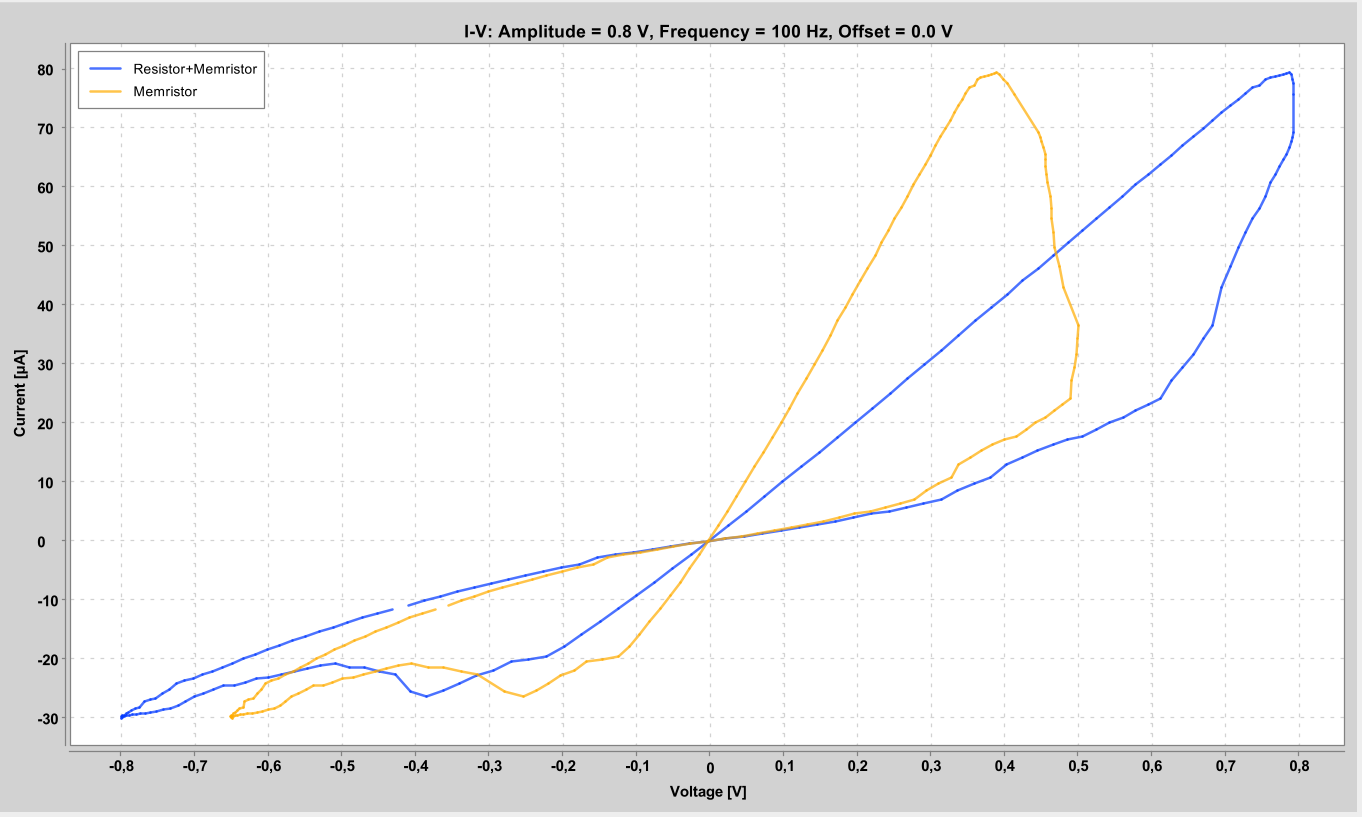
\includegraphics[width=0.85\textwidth]{images/Threshold_Hysterese1.png}
  \caption{Hysterese eines Memristors mit unklarem Forward Threshold.}
  \label{fig:Hysteresen_Threshold}
\end{figure}

Da der Threshold in der Implementierung automatisch aus der Hystere ausgelesen wird, kann dies ein Faktor für die eher niedrigen Noten sein. Der Forward Threshold wird in der Implementierung ausgelesen, indem der erste Punkt in Teil $f_1$ gesucht wird, bei dem das Wachstum der Stromstärke zum nächsten Punkt um 50\% steigt. In Abbildung~\ref{fig:Hysteresen_Threshold} ist zu erkennen, dass die Hysterese bei ungefähr $0.22$V ein erhöhtes Wachstum der Stromstärke verzeichnet. Doch steigt die Hysterese an dieser Stelle noch nicht sofort stark an, sodass nicht mit Sicherheit gesagt werden kann, dass das Wachstum auch die 50\% Marke erreicht. Erst bei $0.32$V kann klar davon ausgegangen werden, dass die Steigung so hoch ist, dass in der Implementierung hier der Threshold gefunden wurde. Das würde die Note für den Forward Threshold in diesem Beispiel fälschlicherweise von 2 auf 4 verschlechtern.

Ein anderer möglicher Grund für eher durchschnittliche Noten für den Energieverbrauch ist die Tatsache, dass die Note aus zwei Teilnoten und ihrem Durchschnitt entsteht. Es wird einerseits der Forward Threshold und andererseits der Reverse Threshold betrachtet und jeweils mit einer Note versehen. Die Gesamtnote aus diesen beiden Teilnoten bildet dann die t-Grade. Wie in Abbildung~\ref{fig:Hysteresen_Threshold} zu erkennen ist, kann eine schlechtere Note für den Reverse Threshold eine bessere Note für den Forward Threshold ausgleichen. In der Abbildung ist der Forward Threshold bei ungefähr $0.22V$ abzulesen, für den Reverse Threshold liegt dieser bei $-0.25$V. Die Noten wären damit für den Forward Threshold bei 2 und für den Reverse Threshold bei 4. Die Gesamtnote für den Threshold würde also bei 3 liegen.

\begin{figure}
  \centering
    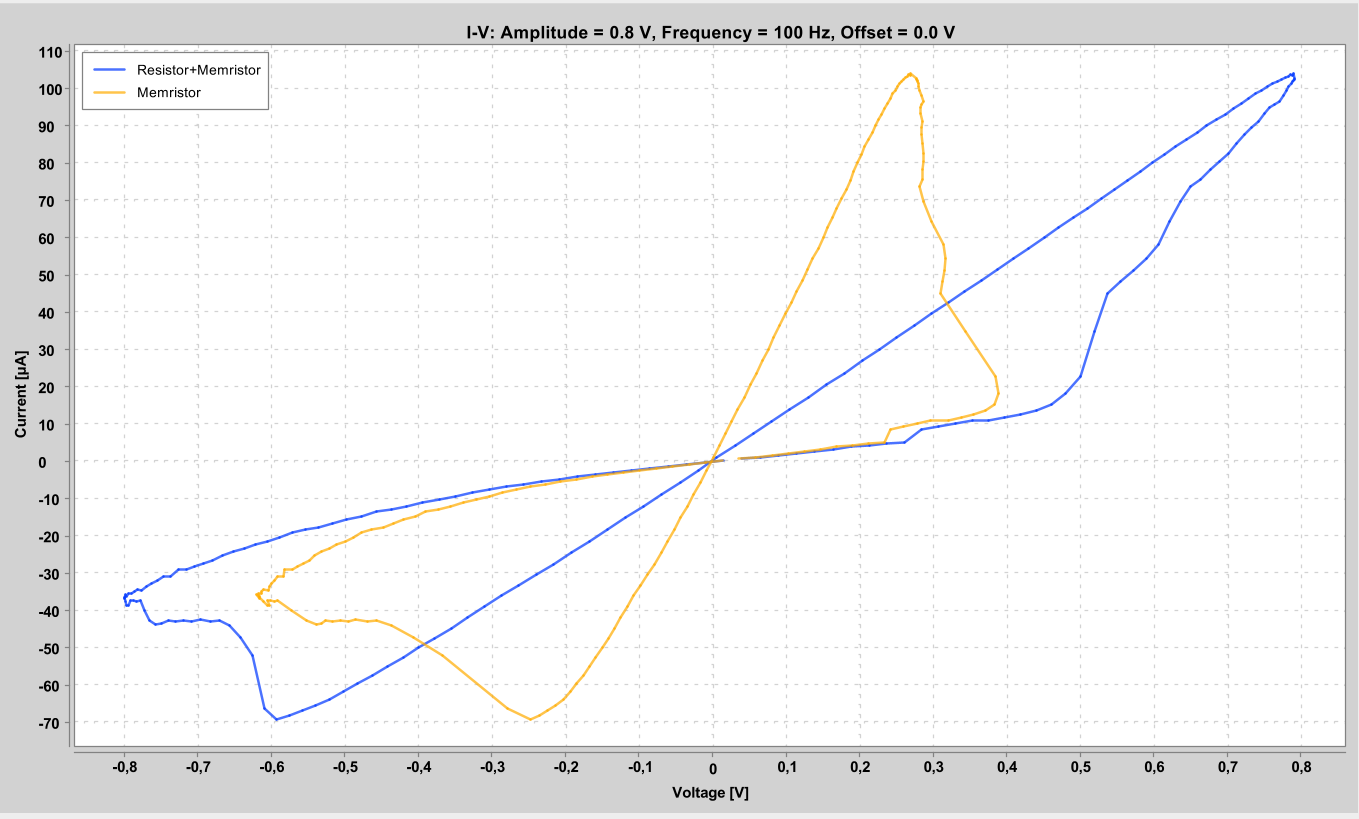
\includegraphics[width=0.85\textwidth]{images/Threshold_Hysterese2.png}
  \caption{Hysterese eines Memristors mit niedrigem Forward Threshold (gut) und niedrigem Reverse Threshold (schlecht).}
  \label{fig:Hysteresen_Threshold2}
\end{figure}

\section{Die Benotung der Speichergrößen}
Dieser Abschnitt wird sich mit den Messungen für die Note zur Speichergröße von Memristoren, der \glqq s-Grade\grqq\,beschäftigen. Auffällig sind hier die über alle Messungen gleichermaßen schlechten und vor allem inkonsistenten Noten für die Speichergrößen, wie in den Tabellen~\ref{tab:Messergebnisse_Sn},~\ref{tab:Messergebnisse_W},~\ref{tab:Messergebnisse_Cr}~und~\ref{tab:Messergebnisse_old}
zu erkennen ist. Wie bereits im Kapitel~\ref{sec:Chapter4} beschrieben wurde, musste für die Implementierung ein anderer Ansatz gewählt werden, als der im Konzept in Kapitel~\ref{sec:Chapter3} vorgestellte Ansatz über Pulse. Da Pulse aus unersichtlichen Gründen mit der Memristor Discovery Software nicht funktionieren, sind auch die Ergebnisse, welche mit dem Ansatz der Berechnung der Leitfähigkeit arbeiten, sehr ungenau und inkonsistent. In der aktuellen Implementierung ist es nicht möglich den Memristor in sein HRS zu bringen, somit ist in den meisten Messungen vermutlich nicht der komplette Wertebereich abgedeckt.

Auch ist der sogenannten \glqq Pulsetrain\grqq, welcher durch die von Knowm gestellte Implementierung übernommen wurde, nicht davor geschützt, dass Memristoren \glqq durchbrennen\grqq, wie es der pulsbasierte Ansatz macht. Wenn nach jedem händischen Puls eine Anzeige des aktuellen Zustands gegeben wird, ist dies auch nicht notwendig. In einem vollständig automatisierten Vorgang, wie bei der Notengeneration dieser Arbeit, kann dies jedoch zu Problemen führen, weshalb aus Vorsicht ein Counter eingebaut wurde, welcher bis zu 10 Pulse erlaubt, bei welchem sich die berechneten Leitfähigkeiten nicht merklich ändern. Danach wird der Vorgang automatisch abgebrochen. Hierbei können auch weitere Zustände \glqq übersehen\grqq\,werden.

\begin{table}
  \centering
    \begin{tabular}{l|c|c|c|c|c|c|c}
      \textbf{Mem.} & \textbf{f-Grade} & \textbf{t-Grade} & \textbf{s-Grade} & \textbf{Grade} & \textbf{minLT} & \textbf{typLT} & \textbf{maxLT} \\\hline
      Cr1          &  3               & 3                &  2               &  2.6           & Inf            & Inf            & Inf     \\
      Cr1          &  1               & 2                &  3               &  3.0           & 503173         & 1807546        & 90361405\\
      Cr1          &  3               & 4                &  2               &  3.0           & Inf            & Inf            & Inf     \\
      Cr1          &  1               & 3                &  4               &  3.6           & -8             & -421           & -842    \\
      Cr1          &  3               & 3                &  3               &  4.0           & 17             & 864            & 1729    \\
      Cr1          &  3               & 3                &  3               &  4.0           & 28450          & 1422871        & 2857942 \\
      Cr1          &  3               & 5                &  3               &  4.6           & 264            & 13248          & 26497   \\
      Cr1          &  4               & 5                &  3               &  5.0           & -17            & -852           & -1704   \\
      Cr1          &  3               & 4                &  3               &  4.6           & 95             & 4768           & 9536    \\
      Cr1          &  3               & 2                &  3               &  2.6           & 28840          & 1442041        & 2884083 \\
      Cr1          &  1               & 3                &  3               &  2.3           & Inf            & Inf            & Inf     \\
      Cr1          &  2               & 3                &  3               &  2.6           & Inf            & Inf            & Inf     \\
      Cr1          &  1               & 3                &  3               &  2.3           & Inf            & Inf            & Inf     \\
      Cr1          &  2               & 2                &  2               &  2.0           & Inf            & Inf            & Inf     \\
    \end{tabular}
  \caption{Ausschnitt der Messergebnisse von wiederholten Messungen auf einem Chrom (Cr) Memristor der neuen Generation.}
  \label{tab:Messergebnisse_Cr}
\end{table}

Ein weiterer Grund für schlechte Noten ist die allgemein sehr strenge Benotung der Speichergrößen. Selbst bei einem vollständig funktionsfähigen und getesteten Ansatz zur Speichergrößenbestimmung wäre nicht sicher, ob einer der Knowm Memristoren 16 oder mehr Zustände erreichen kann. Die meisten aktuellen Memristoren von Knowm können aus Erfahrung in händischen Test zwischen 2.5 und 3.5 Bit codieren. Mehr als 16 Zustände wären bereits in der vier Bit Reichweite, was ein im Vergleich zum Durchschnitt wirklich guten Memristor darstellen würde.

Des Weiteren ist hier bereits etwas anzumerken, was im folgenden Abschnitt~\ref{sec:Restlebensdauer} noch näher beschrieben werden soll. Der Unterschied zwischen dem gemessenen HRS und LRS ist für nahezu alle Messreihen sehr nahe aneinander, manchmal sogar negativ. Das wirft jedoch die Frage auf, wie der leitfähigkeitsbasierte Ansatz, ohne die Zustände merklich zu ändern, verschiedene Leitfähigkeiten berechnet. Dafür müssten weitere Tests und Messreihen mit dem Ansatz gemacht werden, welche es aus Zeitgründen nicht mehr in diese Arbeit geschafft haben.

\section{Die Restlebensdauer}
\label{sec:Restlebensdauer}
Dieser Abschnitt wird sich mit der Bestimmung der Restlebensdauer von Memristoren beschäftigen. Auch hier ist wie im vorherigen Abschnitt auffällig, dass die approximierte Restlebensdauer der Memristoren sehr stark zwischen den einzelnen Messungen schwankt. Dies lässt sich jedoch nicht direkt auf die Berechnung der approximierten Restlebensdauer zurückführen. Diese wurde in dem Kapitel~\ref{sec:Chapter4} beschrieben und näher erklärt. Damit diese Art von Approximation funktionieren kann, muss jedoch zuerst die Messung des HRS und LRS funktionieren.

Wie in den letzten Abschnitten und Kapiteln mehrfach erwähnt wurde, ist dies aufgrund der nicht funktionierenden Pulse jedoch nicht möglich. In nahezu allen Messungen liegen HRS und LRS dadurch sehr nahe aneinender. In den Fällen, in welchen eine negative Restlebensdauer ausgerechnet und zurückgegeben wird, liegt der LRS anhand der Messung sogar knapp über dem HRS. Dazu kommt noch, dass dadurch, dass die beiden Zustände fast immer sehr nahe aneinander liegen, immer der 10\% Restlebensdauer Bereich erreicht wird, was die Gesamtnote immer um eine Note verschlechtert. Dies ist naürlich nicht der Fall, wenn die Restlebensdauer \glqq Inf\grqq\,ist.


\begin{table}
  \centering
    \begin{tabular}{l|c|c|c|c|c|c|c}
      \textbf{Mem.} & \textbf{f-Grade} & \textbf{t-Grade} & \textbf{s-Grade} & \textbf{Grade} & \textbf{minLT} & \textbf{typLT} & \textbf{maxLT} \\\hline
      oldW1          &  3               & 3                &  5               &  4.6           & -38000         & -77400         & -3871676\\
      oldW1          &  2               & 3                &  5               &  3.3           & Inf            & Inf            & Inf     \\
      oldW1          &  2               & 3                &  5               &  3.3           & Inf            & Inf            & Inf     \\
      oldW1          &  4               & 4                &  5               &  5.3           & 996657         & 19993315       & 999665757\\
      oldW1          &  3               & 2                &  5               &  3.3           & Inf            & Inf            & Inf     \\
      oldW1          &  1               & 3                &  5               &  3.0           & Inf            & Inf            & Inf     \\
      oldW1          &  3               & 3                &  5               &  4.6           & 0              & 0              & 0    \\
      oldW1          &  2               & 3                &  5               &  3.3           & Inf            & Inf            & Inf     \\
      oldW1          &  1               & 3                &  6               &  4.3           & 14860          & 29720          & 1486036 \\
      oldW2          &  4               & 3                &  6               &  4.3           & Inf            & Inf            & Inf     \\
      oldW2          &  4               & 3                &  6               &  4.3           & Inf            & Inf            & Inf     \\
      oldW2          &  4               & 3                &  6               &  4.3           & Inf            & Inf            & Inf     \\
      oldW2          &  4               & 3                &  6               &  4.3           & Inf            & Inf            & Inf     \\
      oldW2          &  4               & 3                &  6               &  5.3           & -5944          & -11889         & -594456 \\
    \end{tabular}
  \caption{Ausschnitt der Messergebnisse von wiederholten Messungen auf Wolfram (W) Memristoren der alten Generation.}
  \label{tab:Messergebnisse_old}
\end{table}

Es fällt bei den Messungen auf, dass einige Angaben der Restlebensdauer mit der Bezeichnung \glqq Inf\grqq\,angegeben sind. Dies geschieht nicht in der Konsole und Ausgabe des Programms. \glqq Inf\grqq\,ist in den Tabellen dieses Kapitels vielmehr eine Abkürzung der Zahl $9223372036854775807$, welche für die minimalen, typischen und maximalen Restlebensdauer in der Konsole ausgegeben wird. Da $5000000000$ als maximale Restlebensdauer definiert ist, kann eine solche Restlebensdauer nach Berechnungsvorschrift gar nicht zustande kommen. Wieso sie dann trotzdem angezeigt wird, klärt der folgende Absatz.

Die durch die Memristor Discovery Software gegebene Funktion mit dem Namen \lstinline[columns=fixed]{getSwitchResistancekOhm}
gibt den aktuellen Widerstand des mittels eines \glqq Switch-Buttons\grqq\,ausgewählten Memristors wieder. Der zurückgegebene Widerstand wird jedoch in einigen nicht ersichtlichen Fällen, am häufigsten jedoch, wenn der Memristor in einen hochohmigeren Bereich liegt, nicht als spezifischer Wert, sondern als \glqq Infinity\grqq\,zurückgegeben. Ist dies der Fall, wenn HRS oder LRS gemessen werden, so wird die Berechnung der Restlebensdauer mit \glqq Unendlich\grqq\,als Eingabe berechnet. Bei der Berechnung kommt also in Folge daraus wieder Unendlich heraus, welches mit $9223372036854775807$ ausgegeben wird, da die Restlebensdauer als Datentyp Long gespeichert wird und es sich dabei um den maximalen Wert eines Longs handelt.

\begin{table}
  \centering
    \begin{tabular}{l|c|c||l|c|c}
      \textbf{Mem.} & \textbf{Note} & \textbf{Zeit (in s)} & \textbf{Mem.} & \textbf{Note} & \textbf{Zeit (in s)} \\
      Sn            & 2.3           & 7,46                 & Cr            & 3.3           & 6,12     \\
      Sn            & 4.3           & 9,83                 & Cr            & 3.3           & 8,38     \\
      Sn            & 3.6           & 9,02                 & Cr            & 3.6           & 8,43     \\
      Sn            & 4.6           & 6,35                 & Cr            & 3.3           & 6,50     \\
      Sn            & 4.3           & 7,72                 & Cr            & 1.6           & 7,40     \\
      Sn            & 3.0           & 5,59                 & Cr            & 2.6           & 5,86     \\
      Sn            & 4.0           & 10,26                & Cr            & 3.3           & 8,69     \\
      Sn            & 2.6           & 5,89                 & Cr            & 3.6           & 7,13     \\
      Sn            & 5.0           & 5,86                 & Cr            & 1.6           & 9,10     \\
      Sn            & 4.0           & 9,07                 & Cr            & 3.3           & 6,40     \\
      Sn            & 3.6           & 7,96                 & Cr            & 1.6           & 6,55     \\
      Sn            & 4.0           & 9,50                 & Cr            & 2.0           & 6,82     \\
      Sn            & 4.6           & 6,29                 & Cr            & 2.6           & 8,29     \\
      Sn            & 3.6           & 9,39                 & Cr            & 3.6           & 6,65     \\
      Sn            & 4.3           & 5,28                 & Cr            & 1.6           & 7,13     \\
      Sn            & 3.3           & 7,53                 & Cr            & 3.6           & 5,66     \\
      Sn            & 3.0           & 10,93                & Cr            & 3.3           & 7,67     \\
      Sn            & 4.3           & 10,65                & Cr            & 3.3           & 6,59     \\
      Sn            & 4.6           & 9,65                 & Cr            & 3.3           & 6,78     \\
      Sn            & 4.6           & 7,45                 & Cr            & 2.6           & 6,97     \\
      Sn            & 4.3           & 9,45                 & Cr            & 2.6           & 6,33     \\
      Sn            & 4.6           & 7,56                 & Cr            & 2.0           & 7,91     \\
      Av.           & 3.9           & 8,12                 & Av.           & 2.8           & 7,15     \\
    \end{tabular}
  \caption{Laufzeit eines Durchlaufs zur Qualitätsbestimmung von Memristoren vom Material Zinn und Chrom der neuen Generation.}
  \label{tab:Laufzeit}
\end{table}

Für den Fall, dass sowohl das pulsbasierte Finden von HRS und LRS funktioniert und es einen Weg gibt, den Widerstand des Memristors als konkreten Wert zurückzugeben anstatt in einigen Fällen \glqq Inf\grqq\,als Messung zu erhalten, müsste für die Lebensdauer von Memristoren noch einige Messungen und Test durchgeführt werden. Dabei müsste überprüft werden, ob sich die approximierte Restlebensdauer des Memristors durch wiederholtes Schreiben über einen längeren Zeitraum verringert. Im aktuellen Zustand der Implementierung ist dies noch nicht möglich.

Auch lässt sich über den Zusammenhang zwischen Lebensdauer und Qualität keine Aussage treffen, da die Messergebnisse aus genannten Gründen nicht aussagekräftig genug sind.

\section{Die Laufzeit der Implementierung}

Dieser Abschnitt wird sich mit dem Laufzeit der Implementierung auseinandersetzen. Aus der Messreihe in Tabellen~\ref{tab:Laufzeit}~und~\ref{tab:Laufzeit2} ist zu erkennen, dass sich die Zeit zwischen den Durchläufen teilweise sehr stark unterscheidet. Auffallend ist die erste Messung mit dem Wolframmemristor der neuen Generation. Die $20.39$s, welche dabei benötigt wurden, sind mit großem Abstand die am längsten benötigte Zeit. Dabei handelt es sich um die erste Messung der gesamten Messreihe über alle Memristorarten. Es konnte jedoch noch nicht rekonstruiert werden, ob die erste Messung auf den Memristoren immer länger dauert, als die nachfolgenden Messungen.

Auffällig ist außerdem, dass die durchschnittliche Dauer der Qualitätsbestimmung für die Chrom Memristoren eindeutig am niedrigsten von allen Memristortypen ist. Daraus lässt sich folgern, dass Chrom Memristoren dafür, dass sie einen höheren Threshold und eine kürzere Gesamtlebensdauer haben (siehe~\cite{knowm_comp_2019}), eine schnellere Lese- und Schreibgeschwindigkeit besitzen.

\begin{table}
  \centering
    \begin{tabular}{l|c|c||l|c|c}
      \textbf{Mem.} & \textbf{Note} & \textbf{Zeit (in s)} & \textbf{Mem.} & \textbf{Note} & \textbf{Zeit (in s)} \\
      W$_{\text{new}}$            & 4.0           & 20,39                & W$_{\text{old}}$            & 4.3           & 5,75     \\
      W$_{\text{new}}$            & 3.3           & 12,79                & W$_{\text{old}}$            & 5.3           & 9,48     \\
      W$_{\text{new}}$            & 4.0           & 14,53                & W$_{\text{old}}$            & 5.0           & 5,08\footnote{\label{tab_footnote}Vorzeitiger Abbruch (Programm wurde nicht vollständig durchgeführt)}     \\
      W$_{\text{new}}$            & 3.3           & 10,96                & W$_{\text{old}}$            & 5.3           & 8,58     \\
      W$_{\text{new}}$            & 3.6           & 12,36                & W$_{\text{old}}$            & 3.0           & 8,42     \\
      W$_{\text{new}}$            & 3.3           & 8,88                 & W$_{\text{old}}$            & 4.3           & 7,43     \\
      W$_{\text{new}}$            & 2.0           & 7,88                 & W$_{\text{old}}$            & 3.0           & 7,90     \\
      W$_{\text{new}}$            & 3.0           & 4,65                 & W$_{\text{old}}$            & 4.3           & 11,30    \\
      W$_{\text{new}}$            & 1.6           & 8,02                 & W$_{\text{old}}$            & 4.3           & 10,78    \\
      W$_{\text{new}}$            & 3.3           & 7,55                 & W$_{\text{old}}$            & 5.3           & 8,63     \\
      W$_{\text{new}}$            & 2.3           & 7,23                 & W$_{\text{old}}$            & 5.3           & 6,52     \\
      W$_{\text{new}}$            & 3.0           & 8,53                 & W$_{\text{old}}$            & 4.3           & 10,09    \\
      W$_{\text{new}}$            & 3.3           & 10,05                & W$_{\text{old}}$            & 3.6           & 14,26    \\
      W$_{\text{new}}$            & 3.3           & 5,42                 & W$_{\text{old}}$            & 3.3           & 7,03     \\
      W$_{\text{new}}$            & 4.0           & 6,09                 & W$_{\text{old}}$            & 5.3           & 6,83     \\
      W$_{\text{new}}$            & 1.6           & 6,18                 & W$_{\text{old}}$            & 3.6           & 9,43     \\
      W$_{\text{new}}$            & 3.0           & 8,20                 & W$_{\text{old}}$            & 3.6           & 10,03    \\
      W$_{\text{new}}$            & 3.6           & 7,62                 & W$_{\text{old}}$            & 4.0           & 8,43     \\
      W$_{\text{new}}$            & 3.6           & 9,83                 & W$_{\text{old}}$            & 5.3           & 8,23     \\
      W$_{\text{new}}$            & 3.6           & 9,26                 & W$_{\text{old}}$            & 5.0           & 7,68\footref{tab_footnote}     \\
      W$_{\text{new}}$            & 2.0           & 7,20                 & W$_{\text{old}}$            & 5.0           & 2.16\footref{tab_footnote}     \\
      W$_{\text{new}}$            & 3.6           & 8,18                 & W$_{\text{old}}$            & 4.0           & 8,55     \\
      Av.                         & 3.1           & 9,17                 & Av.                         & 4.3           & 8,20     \\
    \end{tabular}
  \caption{Laufzeit eines Durchlaufs zur Qualitätsbestimmung von Memristoren vom Material Wolfram der neuen und alten Generation.}
  \label{tab:Laufzeit2}
\end{table}

Für alle Memristortypen lässt sich aus den Tabellen~\ref{tab:Laufzeit}~und~\ref{tab:Laufzeit2} außerdem entnehmen, dass die Note keinerlei Einfluss auf die Laufzeit des Programms hat. Trotzdem ist die Zeit, wie bereits beschrieben, sehr unterschiedlich in den verschiedenen Messungen. Dies lässt sich darauf zurückführen, dass es im Programm öfter zu Wiederholungen von Messungen kommt, wenn diese unvollständig oder verschoben aufgenommen werden. Nur wenn eine Messung mehrmals hintereinander fehlschlägt, wird abgebrochen. Die Folge daraus ist, dass bei einigen Messungen eine erhöhte Anzahl an Messwiederholungen stattfinden. Wenn ein funktionierender Memristor vorliegt, wird im Fall, dass die Messung fehlschlägt, in einer der darauf folgenden Messwiederholungen eine valide Messung vorgenommen und der Vorgang zur Qualitätsbestimmung kann weiter durchgeführt werden. In Folge dessen steigt die Bearbeitungszeit jedoch an. Somit entstehen sehr unterschiedliche Bearbeitungszeiten für die verschiedenen Messungen auf den Memristortypen.

\section{Der Einfluss des Materials auf die Qualität}
In diesem Abschnitt soll es abschließend um den Einfluss des Materials auf die Qualität gehen. Aufgrund der in diesem Kapitel beschriebene Probleme, können keine klaren Aussagen über den Einfluss des Materials auf die Qualität getroffen werden. Doch ist auffällig, dass der Zinnmemristor in Tabelle~\ref{tab:Laufzeit} von der durchschnittlichen Qualität der Messreihe eher dem Memristor der alten Generation ähnelt, während die Memristoren aus dem Material Chrom aus Tabelle~\ref{tab:Laufzeit} und dem Material Wolfram der neuen Generation aus Tabelle~\ref{tab:Laufzeit2} mit ihrer durchschnittlichen Qualität näher aneinander liegen. Auch fällt auf, dass die durchschnittliche Laufzeit zum Kategorisieren der Memristoren für die Wolfram Memristoren beider Generationen und für den Zinn Memristor ähnlich lange ist. Der Wolfram Memristor der neuen Generation sticht durch die ungewöhnlich lange Messung zu Beginn zwar im Durchschnitt mit fast einer Sekunde heraus, wenn der Durchschnitt jedoch aus den anderen 21 Messwerten errechnet wird und die 20,39s zu Beginn ignoriert werden, errechnet sich eine durchschnittliche Laufzeit von 8,6s. Der Chrom Memristor dagegen scheint mit keiner einzigen Laufzeit von über 10 Sekunden und einem Durchschnitt von 7,15s schneller als die Memristoren anderer Materialen zu sein.
